% Compilar en Overleaf con pdfLaTeX
% Proyecto: HarmoniWatts — Tarea Arquitectura de Información (Act. 11)
\documentclass[11pt,a4paper]{article}

\usepackage[utf8]{inputenc}
\usepackage[T1]{fontenc}
\usepackage[spanish,es-tabla]{babel}
\usepackage{geometry}
\usepackage{array}
\usepackage{tabularx}
\usepackage{longtable}
\usepackage{booktabs}
\usepackage{multirow}
\usepackage{makecell}
\usepackage{ragged2e}
\usepackage{xcolor}
\usepackage{colortbl}
\usepackage{hyperref}
\usepackage{float}
\usepackage{enumitem}
\usepackage{graphicx}
\graphicspath{{../imagenes/diagramas/}}
\usepackage{tikz}
\usetikzlibrary{shapes,arrows.meta,positioning,fit,calc}

\geometry{margin=2.2cm}
\hypersetup{colorlinks=true, linkcolor=blue!60!black, urlcolor=blue!60!black}

\definecolor{tabhead}{gray}{0.88}
\colorlet{impl}{green!45!black}
\colorlet{plan}{orange!70!black}
\newcolumntype{L}[1]{>{\RaggedRight\arraybackslash\hspace{0pt}}p{#1}}
\newcolumntype{Y}{>{\RaggedRight\arraybackslash\hspace{0pt}}X}
\renewcommand{\arraystretch}{1.2}
\setlength{\tabcolsep}{4pt}

\newcommand{\stimpl}{\textcolor{impl}{\textbf{[Impl.]}}}
\newcommand{\stplan}{\textcolor{plan}{\textbf{[Plan.]}}}
\newcommand{\stelim}{\textbf{[Elim.]}}

\title{\textbf{Tarea: Arquitectura de Información}\\
\large HarmoniWatts --- Diagramas, descripciones y justificaciones (parte A)}
\author{Christian Camilo Rosero Rodríguez \\ Carlos David Rojas Lozano}
\date{Mayo 2026}

\begin{document}
\maketitle

\begin{center}
\small
\textbf{Maestría Virtual en Ingeniería de Sistemas y Computación}\\
Profesor: Javier Mauricio Reyes Vera Ph.D.
\end{center}

\vspace{0.5em}
\noindent\textbf{Aplicación:} HarmoniWatts --- HEMS para optimizar consumo eléctrico residencial frente a tarifas horarias (TOU) con predicción y recomendaciones IA.

\vspace{0.8em}
\noindent\textbf{Referencias del proyecto:} BPM del proceso HEMS, arquitectura técnica del repositorio y contrato REST del dashboard.

\vspace{0.5em}
\begin{tabular}{@{}L{2.2cm}L{12cm}@{}}
\toprule
\textbf{Símbolo} & \textbf{Significado} \\
\midrule
\stimpl & Implementado en el repositorio (Angular + servicios actuales) \\
\stplan & Planificado en backlog; navegación visible como ``próximamente'' \\
\stelim & Eliminado del mapa respecto al diseño inicial \\
\bottomrule
\end{tabular}

\section{Descripción de la aplicación}

HarmoniWatts es una aplicación web que ayuda a hogares colombianos a \textbf{entender su consumo eléctrico}, \textbf{anticipar costos} según franjas tarifarias y \textbf{actuar sobre recomendaciones de ahorro} generadas por IA. El flujo de negocio principal ---modelado en el BPM del proyecto--- conecta cinco actores:

\begin{enumerate}[leftmargin=*]
  \item \textbf{Usuario:} crea cuenta, ingresa al sistema y decide si aplica o descarta un consejo de ahorro.
  \item \textbf{La aplicación:} muestra el panel de consumo y los consejos.
  \item \textbf{Contador inteligente:} lee y persiste el consumo del hogar.
  \item \textbf{Tarifas eléctricas:} actualizan automáticamente las franjas del día (CREG / comercializador).
  \item \textbf{Inteligencia artificial:} predice consumo y calcula el mejor horario para aparatos desplazables.
\end{enumerate}

\textbf{Usuario objetivo:} persona residencial con factura regulada por franjas horarias, interesada en reducir costo sin perder confort. No hay rol administrador ni comercializador en la UI actual.

\textbf{Alcance:} refleja lo \textbf{ya construido} (auth, dashboard, cuenta/perfil, vivienda, electrodomésticos) y deja módulos futuros \textbf{acotados}, evitando duplicar contenido entre pantallas.

\subsection{Proceso de negocio (BPM)}

El mapa del sitio se alinea con el flujo BPMN del HEMS. A continuación, el diagrama del proceso (cinco carriles: Usuario, Aplicación, Contador, Tarifas e IA).

\begin{figure}[H]
\centering
% Sube a Overleaf el PNG exportado desde HarmoniWatts_BPM.drawio
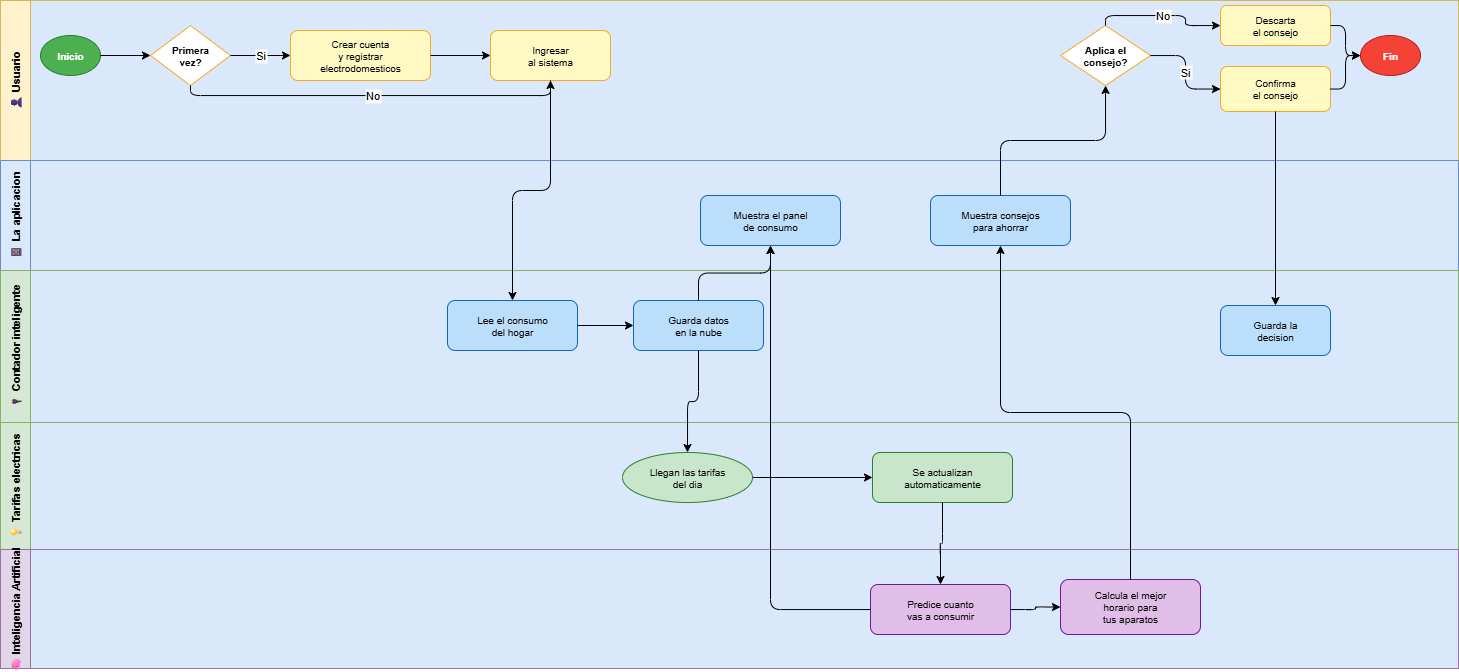
\includegraphics[width=0.92\textwidth]{HarmoniWatts_BPM.png}
\caption{Diagrama BPM --- proceso general HarmoniWatts (BPMN 2.0).}
\end{figure}

\section{Mapa del sitio}

\subsection{Descripción de la estructura}

Se adoptó una \textbf{estructura jerárquica de dos niveles} (módulo $\rightarrow$ sección), con separación clara entre \textbf{zona pública} (sin autenticación) y \textbf{zona privada} (post-login). El criterio organizador de primer nivel es el \textbf{flujo del BPM}: acceder $\rightarrow$ ver panel $\rightarrow$ consultar tarifas $\rightarrow$ recibir y decidir sobre recomendaciones $\rightarrow$ (futuro) revisar reportes.

\begin{table}[H]
\centering
\small
\begin{tabularx}{\textwidth}{@{}L{4.5cm}Y@{}}
\toprule
\textbf{Decisión} & \textbf{Motivo} \\
\midrule
Eliminar \emph{Vista de consumo} en Consumo y tarifas &
El consumo del día (KPIs, gráfico horario, predicción IA y franjas) ya vive en el Dashboard. \\
Eliminar \emph{Simular cambio de tarifa} &
Las tarifas se actualizan automáticamente según el BPM; la simulación no está en alcance del MVP. \\
Acotar Dashboard y Mi perfil (Cuenta) &
Solo se listan secciones con pantalla o API existente en el repositorio. \\
Acotar Reportes &
Se mantienen resumen/exportación y comparativas; se eliminó informes personalizados del MVP. \\
\bottomrule
\end{tabularx}
\caption{Ajustes respecto al mapa del sitio inicial del proyecto}
\end{table}

\begin{figure}[H]
\centering
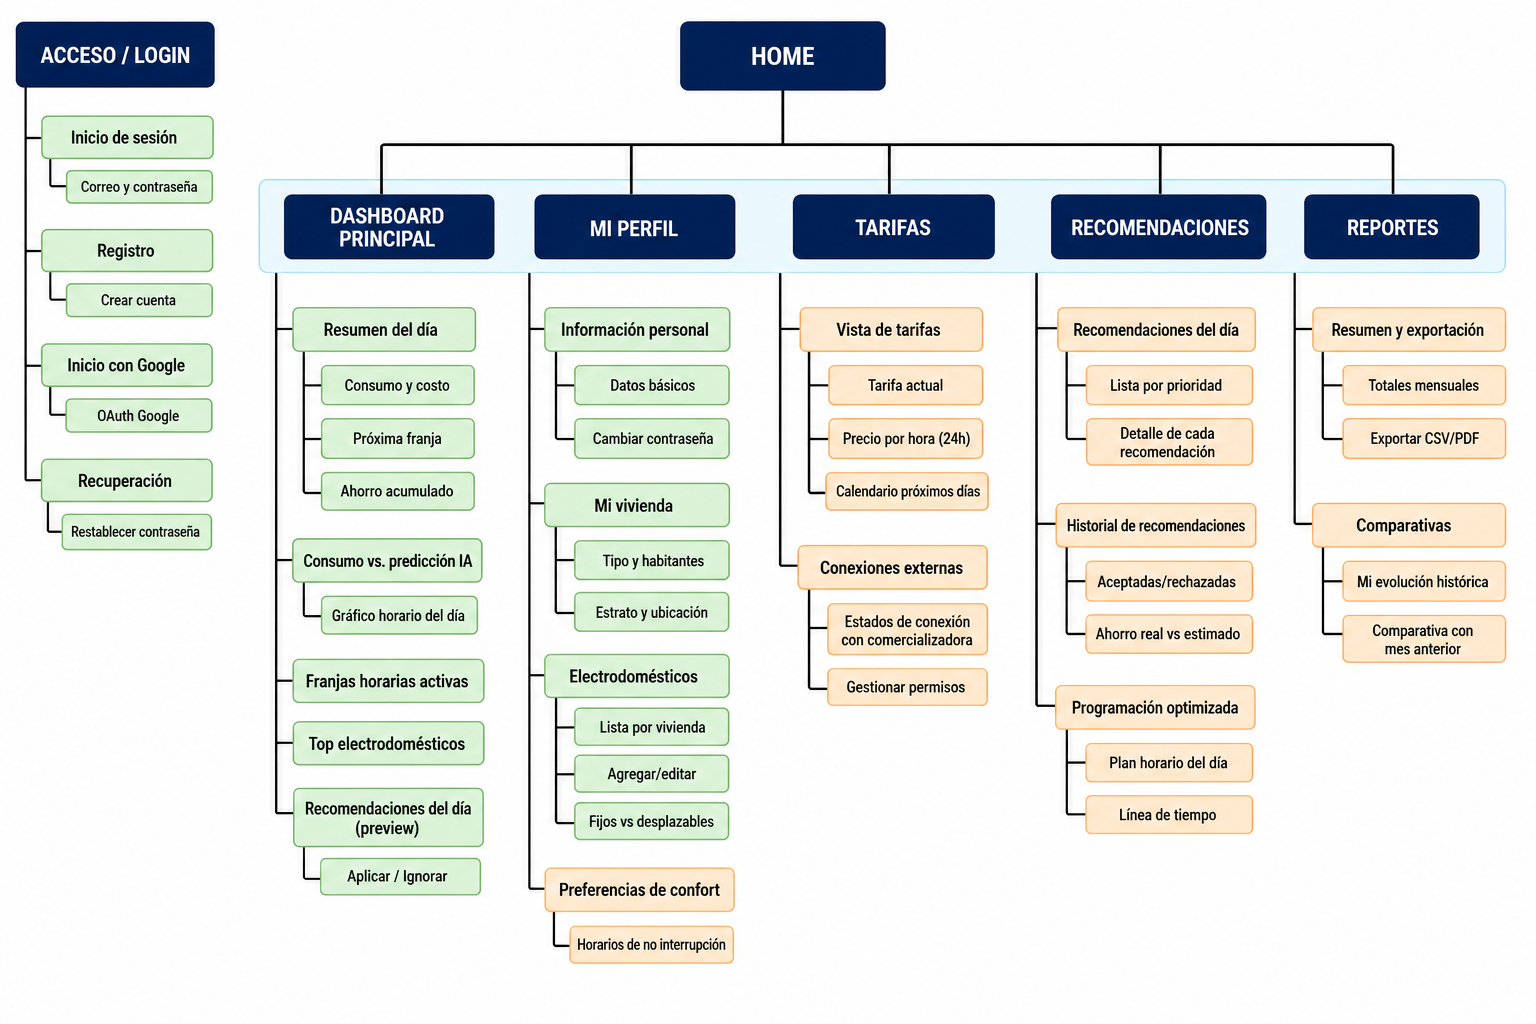
\includegraphics[width=\textwidth]{HarmoniWatts_MapaSitio.png}
\caption{Mapa del sitio HarmoniWatts. \textbf{Verde:} secciones implementadas; \textbf{naranja:} planificadas en backlog.}
\end{figure}

\subsection{Tabla detallada del mapa del sitio}

{\scriptsize
\begin{longtable}{@{}L{2.4cm}L{2.2cm}L{3.8cm}L{1.1cm}L{3.2cm}@{}}
\toprule
\textbf{Nivel 1} & \textbf{Nivel 2} & \textbf{Nivel 3 / acciones} & \textbf{Est.} & \textbf{Ruta / notas} \\
\midrule
\endfirsthead
\toprule
\textbf{Nivel 1} & \textbf{Nivel 2} & \textbf{Nivel 3 / acciones} & \textbf{Est.} & \textbf{Ruta / notas} \\
\midrule
\endhead
0. Acceso / Login & 0.1 Inicio de sesión & Correo + contraseña & \stimpl & \texttt{/auth/login} \\
 & 0.2 Registro & Formulario; verificación email & \stimpl & \texttt{/auth/register} \\
 & 0.3 Inicio con Google & OAuth vía Keycloak (\texttt{idpHint}) & \stimpl & Botón en login \\
 & 0.4 Recuperación & Enlace por correo & \stimpl & \texttt{/auth/forgot-password} \\
\midrule
1. Dashboard & 1.1 Resumen del día & Consumo, costo, ahorro, próxima franja & \stimpl & \texttt{/dashboard} \\
 & 1.2 Consumo vs. IA & Gráfico horario; selector fecha & \stimpl & API consumption-chart \\
 & 1.3 Franjas activas & Bandas Valle / Media / Punta & \stimpl & Panel lateral \\
 & 1.4 Top electrodomésticos & Ranking del día & \stimpl & API appliances-top \\
 & 1.5 Reco. (preview) & Aplicar / Ignorar & \stimpl & Tarjetas en dashboard \\
\midrule
2. Mi perfil & 2.0 Hub Cuenta & Tarjetas de acceso & \stimpl & \texttt{/cuenta} \\
 & 2.1 Información personal & Datos básicos; cambiar contraseña & \stimpl & \texttt{/perfil/editar/*} \\
 & 2.2 Mi vivienda & Tipo, habitantes, estrato, ubicación & \stimpl & \texttt{/mi-vivienda} \\
 & 2.3 Electrodomésticos & Lista, agregar/editar, fijos vs desplazables & \stimpl & \texttt{/cuenta/electrodomesticos} \\
 & 2.4 Pref. confort & Horarios de no interrupción & \stplan & Próximamente en hub \\
\midrule
3. Tarifas & 3.1 Vista tarifas & Tarifa actual; precio 24 h; calendario & \stplan & Sidebar deshabilitado \\
 & 3.2 Conexiones externas & Estado con comercializadora; permisos & \stplan & Integración futura \\
 & Vista de consumo & --- & \stelim & Ver módulo 1 \\
 & Simular tarifa & --- & \stelim & Fuera del BPM \\
\midrule
4. Recomendaciones & 4.1 Reco. del día & Lista por prioridad; detalle & \stplan & Módulo completo \\
 & 4.2 Historial & Aceptadas/rechazadas; ahorro real vs estimado & \stplan & Complementa preview \\
 & 4.3 Programación & Plan horario; línea de tiempo & \stplan & ``Mejor horario'' BPM \\
\midrule
5. Reportes & 5.1 Resumen y export. & Totales mensuales; CSV/PDF & \stplan & Módulo futuro \\
 & 5.2 Comparativas & Evolución histórica; vs mes anterior & \stplan & Análisis longitudinal \\
\bottomrule
\end{longtable}
}

\subsection{Justificación del mapa del sitio}

\begin{itemize}[leftmargin=*]
  \item \textbf{Dashboard como hub operativo único de consumo.} El BPM indica que, tras guardar datos del contador, la aplicación ``muestra el panel de consumo''. Concentrar KPIs, serie horaria, franjas y ranking en un solo módulo reduce saltos de navegación en el uso diario.
  \item \textbf{Módulo Tarifas enfocado en precio, no en kWh.} Separar precio (consulta tarifaria) de consumo (medición) respeta el carril ``Tarifas eléctricas'' del BPM.
  \item \textbf{Cuenta como agrupador del hogar.} Vivienda y electrodomésticos corresponden al paso ``Crear cuenta y registrar electrodomésticos'' del BPM en primer uso.
  \item \textbf{Eliminación de simulación de tarifa.} Contradice el flujo automático del BPM y no aporta valor cuando la fuente tarifaria es externa y de solo lectura.
\end{itemize}

\begin{table}[H]
\centering
\small
\begin{tabularx}{\textwidth}{@{}L{4.2cm}L{4.2cm}@{}}
\toprule
\textbf{Paso BPM} & \textbf{Ubicación en el mapa} \\
\midrule
Crear cuenta / ingresar & Módulo 0 \\
Registrar electrodomésticos & 2.3 (vía 2.2 si no hay vivienda) \\
Panel de consumo & Módulo 1 completo \\
Tarifas del día & 1.3 + 1.1 + módulo 3 \stplan \\
Predicción IA & 1.2 \\
Consejos para ahorrar & 1.5 (+ módulo 4 \stplan) \\
¿Aplica el consejo? & 1.5 Aplicar / Ignorar \\
Guarda la decisión & Backend; historial \stplan \\
\bottomrule
\end{tabularx}
\caption{Correspondencia BPM $\leftrightarrow$ mapa del sitio}
\end{table}

\section{Taxonomías y metadatos}

\subsection{Taxonomía de franjas tarifarias (TOU)}

Clasificación \textbf{jerárquica exclusiva} por intervalo horario. Cada hora pertenece a una sola franja.

\begin{table}[H]
\centering
\small
\begin{tabular}{@{}L{3.2cm}L{4.5cm}L{5.5cm}@{}}
\toprule
\textbf{Nivel} & \textbf{Categorías} & \textbf{Ejemplo} \\
\midrule
Tipo de franja & \texttt{VALLE}, \texttt{MEDIA}, \texttt{PUNTA} & 22:00--06:00 $\rightarrow$ VALLE \\
Precio & Numérico (COP/kWh) & 245 COP/kWh en VALLE \\
Ventana temporal & \texttt{startHour}, \texttt{endHour} (0--23) & PUNTA 18:00--22:00 \\
\bottomrule
\end{tabular}
\caption{Taxonomía TOU}
\end{table}

\textbf{Justificación:} Una hora no puede ser Valle y Punta a la vez; la clasificación exclusiva simplifica colores en gráfico y KPI ``Próxima franja''. Implementado en \texttt{TariffBand} / \texttt{TariffType} y contrato REST del dashboard.

\subsection{Taxonomía de electrodomésticos}

Taxonomía \textbf{polijerárquica} en tipos predefinidos + atributos transversales.

\begin{table}[H]
\centering
\small
\begin{tabularx}{\textwidth}{@{}L{2.8cm}L{5.5cm}Y@{}}
\toprule
\textbf{Dimensión} & \textbf{Valores / regla} & \textbf{Ejemplo} \\
\midrule
Tipo predefinido & Catálogo BD + código \texttt{OTRO} & Lavadora, nevera, ``Otro'' \\
Marca & Catálogo + \texttt{OTRO} con texto libre & Samsung / ``Otro: Mabe'' \\
Desplazabilidad & Booleano \texttt{es\_desplazable} & Lavadora desplazable; nevera fija \\
Categoría visual & Derivada del tipo (iconografía) & \texttt{heat}, \texttt{washer}, \texttt{hvac}, \texttt{fridge} \\
\bottomrule
\end{tabularx}
\end{table}

\textbf{Justificación:} Un aparato se filtra por tipo (IA y ranking), desplazabilidad (optimización BPM) y vivienda (multi-hogar) sin duplicar registros.

\subsection{Taxonomía de vivienda}

\begin{table}[H]
\centering
\small
\begin{tabular}{@{}L{2.5cm}L{2.5cm}L{7cm}@{}}
\toprule
\textbf{Campo} & \textbf{Tipo} & \textbf{Valores} \\
\midrule
\texttt{tipo} & Enum UI & Casa, Apartamento, Otro \\
\texttt{estrato} & Entero 1--6 & Estrato socioeconómico Colombia \\
\texttt{habitantes} & Entero & 1--99 \\
\texttt{ubicacion} & Texto & Dirección o referencia \\
\bottomrule
\end{tabular}
\end{table}

\subsection{Metadatos principales}

\subsubsection{Consumo (serie horaria)}

\begin{table}[H]
\centering
\scriptsize
\begin{tabularx}{\textwidth}{@{}L{2.6cm}L{2cm}L{4.5cm}Y@{}}
\toprule
\textbf{Campo} & \textbf{Tipo} & \textbf{Descripción} & \textbf{Uso} \\
\midrule
\texttt{date} & ISO date & Día de medición & Filtro dashboard \\
\texttt{timezone} & String & Zona horaria & Eje temporal \\
\texttt{actualKwh} & Array & Consumo real/hora & Gráfico + KPIs \\
\texttt{predictedKwh} & Array|null & Predicción IA & Línea punteada \\
\texttt{currentHourLocal} & Entero & Hora actual & Marcador vertical \\
\texttt{tariffBands} & Array & Franjas del día & Fondo gráfico \\
\bottomrule
\end{tabularx}
\end{table}

\subsubsection{Recomendación IA}

\begin{table}[H]
\centering
\scriptsize
\begin{tabularx}{\textwidth}{@{}L{2.8cm}L{2.2cm}L{4.2cm}Y@{}}
\toprule
\textbf{Campo} & \textbf{Tipo} & \textbf{Descripción} & \textbf{Uso} \\
\midrule
\texttt{id} & String & Identificador & Apply / dismiss \\
\texttt{title}, \texttt{body} & String & Mensaje al usuario & Tarjeta dashboard \\
\texttt{estimatedSavingsCop} & Numérico & Ahorro estimado & Decisión \\
\texttt{suggestedStart} & DateTime & Horario sugerido & Programación \stplan \\
\texttt{priority} & Entero & Orden visual & Top N \\
\bottomrule
\end{tabularx}
\end{table}

\subsubsection{Electrodoméstico (PostgreSQL)}

\begin{table}[H]
\centering
\scriptsize
\begin{tabularx}{\textwidth}{@{}L{2.6cm}L{1.8cm}L{4.8cm}Y@{}}
\toprule
\textbf{Campo} & \textbf{Tipo} & \textbf{Descripción} & \textbf{Uso} \\
\midrule
\texttt{potencia\_w} & Entero & Potencia nominal & Cálculo de carga \\
\texttt{uso\_semanal} & Entero & Veces por semana & Perfil de uso \\
\texttt{horario\_habitual} & Time & Hora típica & IA / recomendaciones \\
\texttt{es\_desplazable} & Boolean & ¿Movable de franja? & Optimizador BPM \\
\texttt{activo} & Boolean & Incluir en análisis & CRUD \\
\bottomrule
\end{tabularx}
\end{table}

\textbf{Justificación de \texttt{es\_desplazable}:} enlaza con el carril IA del BPM (``Calcula el mejor horario para tus aparatos''). Sin este flag, el optimizador trataría igual una nevera y una lavadora.

\textbf{Justificación de \texttt{predictedKwh} nullable:} si el predictor falla, el dashboard sigue mostrando consumo real (degradación graceful).

\section{Navegabilidad}

\subsection{Sistema de navegación principal}

\begin{table}[H]
\centering
\small
\begin{tabularx}{\textwidth}{@{}L{2.6cm}L{4.2cm}L{2.8cm}Y@{}}
\toprule
\textbf{Sistema} & \textbf{Descripción} & \textbf{Ubicación} & \textbf{Módulos} \\
\midrule
Barra lateral fija & Nav.\ primaria post-login & Columna izquierda & Dashboard \stimpl; Tarifas, Reco., Historial \stplan \\
Hub de tarjetas & Nav.\ secundaria Cuenta & \texttt{/cuenta} & Perfil, vivienda, electrodomésticos \\
Enlaces contextuales & Saltos guiados & Cuerpo de pantallas & Ej.: ``Registra una vivienda'' \\
Breadcrumbs implícitos & Volver a Cuenta & Electrodomésticos & \texttt{/cuenta/electrodomesticos} \\
\bottomrule
\end{tabularx}
\end{table}

\textbf{Justificación:} el Dashboard es destino por defecto (\texttt{'' $\rightarrow$ dashboard}) porque es la pantalla de mayor frecuencia tras login, alineada al BPM (panel de consumo inmediato).

\subsection{Flujo de navegación principal}

\begin{table}[H]
\centering
\small
\begin{tabularx}{\textwidth}{@{}c L{3.2cm}L{3.5cm}Y@{}}
\toprule
\textbf{\#} & \textbf{Pantalla} & \textbf{Decisión} & \textbf{Destino} \\
\midrule
1 & Abrir app & ¿Sesión activa? & Sí $\rightarrow$ Dashboard / No $\rightarrow$ Login \\
2 & Login & ¿Credenciales válidas? & Dashboard o error \\
3 & Registro & ¿Correo verificado? & Login $\rightarrow$ Dashboard \\
4 & Dashboard & --- & KPIs, gráfico, recomendaciones \\
5 & Primer uso & ¿Hay vivienda? & No $\rightarrow$ Cuenta $\rightarrow$ Mi vivienda \\
6 & Vivienda + apps & Datos mínimos IA & Vuelta a Dashboard \\
7 & Recomendación & ¿Aplica consejo? & POST apply / dismiss \\
8 & Fin ciclo & --- & Dashboard o Tarifas \stplan \\
\bottomrule
\end{tabularx}
\end{table}

\begin{figure}[H]
\centering
\small
\begin{tikzpicture}[
  node distance=0.7cm and 1.2cm,
  proc/.style={draw, rounded corners, align=center, minimum width=2.4cm, minimum height=0.7cm, font=\scriptsize},
  dec/.style={draw, diamond, aspect=2, align=center, inner sep=1pt, font=\scriptsize},
  term/.style={draw, circle, align=center, minimum size=0.75cm, font=\scriptsize},
  arr/.style={-{Stealth[length=1.5mm]}, thick}
]
  \node[term] (a) {Inicio};
  \node[dec, below=of a] (b) {¿Auth?};
  \node[proc, left=of b] (l) {Login / Registro};
  \node[proc, below=of b] (d) {Dashboard};
  \node[dec, below=of d] (e) {¿Vivienda?};
  \node[proc, right=of e] (f) {Cuenta $\rightarrow$ Apps};
  \node[dec, below=of e] (g) {¿Reco. IA?};
  \node[proc, below left=of g] (h) {Aplicar};
  \node[proc, below right=of g] (i) {Ignorar};
  \node[term, below=1.1cm of g] (j) {Fin};

  \draw[arr] (a) -- (b);
  \draw[arr] (b) -- node[above, font=\tiny]{No} (l);
  \draw[arr] (l) |- (b);
  \draw[arr] (b) -- node[right, font=\tiny]{Sí} (d);
  \draw[arr] (d) -- (e);
  \draw[arr] (e) -- node[above, font=\tiny]{No} (f);
  \draw[arr] (f) |- (d);
  \draw[arr] (e) -- node[right, font=\tiny]{Sí} (g);
  \draw[arr] (g) -- node[left, font=\tiny]{Sí} (h);
  \draw[arr] (g) -- node[right, font=\tiny]{No} (i);
  \draw[arr] (h) -- (j);
  \draw[arr] (i) -- (j);
\end{tikzpicture}
\caption{Flujo de navegación principal (primer uso y ciclo diario)}
\end{figure}

\textbf{Justificación del flujo post-registro:} el BPM exige registrar electrodomésticos en primer uso, pero no bloquea el login. Equilibrio entre onboarding progresivo y valor temprano (ver consumo con inventario incompleto).

\section{Mecanismos de búsqueda}

HarmoniWatts no es un catálogo masivo; la búsqueda es \textbf{contextual y acotada}.

\begin{table}[H]
\centering
\small
\begin{tabularx}{\textwidth}{@{}L{2.8cm}L{4.5cm}L{2cm}Y@{}}
\toprule
\textbf{Mecanismo} & \textbf{Descripción} & \textbf{Módulo} & \textbf{Método} \\
\midrule
Selector de vivienda & Filtra electrodomésticos & 2.3 & \texttt{<select>} \\
Selector de fecha & Cambia día del dashboard & 1 & \texttt{type=date} + query API \\
Catálogo tipo/marca & Taxonomía predefinida & 2.3 & Select backend \\
Actualizar & Refetch explícito & 1, listas & Botón \\
Búsqueda texto \stplan & Historial / reportes & 4, 5 & Filtro client o API \\
\bottomrule
\end{tabularx}
\end{table}

\subsection{Reglas del selector de fecha (dashboard)}

\begin{enumerate}[leftmargin=*]
  \item Por defecto: fecha local del navegador.
  \item Al cambiar fecha: recarga paralela de summary, chart, recommendations y appliances-top.
  \item Fechas futuras: según reglas del API (422 si no aplicable).
\end{enumerate}

\textbf{Justificación:} la búsqueda principal del usuario es temporal (``¿cómo estuvo ayer?''), no lexical. El volumen de entidades por usuario es bajo (pocas viviendas, decenas de electrodomésticos).

\subsection{Catálogo de electrodomésticos (MVP)}

\begin{enumerate}[leftmargin=*]
  \item Tipos y marcas ordenados (\texttt{orden ASC}) desde PostgreSQL.
  \item Si tipo = \texttt{OTRO}, el nombre es obligatorio (cliente y servidor).
  \item Sin autocompletado full-text; lista corta y escaneable.
\end{enumerate}

\section{Resumen de decisiones de arquitectura de información}

{\scriptsize
\begin{longtable}{@{}L{3.2cm}L{3.2cm}L{3.5cm}L{3.5cm}@{}}
\toprule
\textbf{Decisión} & \textbf{Alternativa descartada} & \textbf{Criterio} & \textbf{Validación} \\
\midrule
Consumo solo en Dashboard & Vista de consumo en Tarifas & Hub operativo único & BPM + código \\
Tarifas sin simulador & Simular cambio tarifa & Tarifas automáticas & BPM \\
Cuenta agrupa perfil + hogar & Mi perfil con 4 ramas & Sidebar simple & \texttt{app.routes.ts} \\
Reco. preview + historial & Solo módulo Reco. & Decisión rápida en dashboard & BPM \\
Taxonomía TOU exclusiva & Etiquetas múltiples/hora & Modelo CREG & \texttt{TariffBand} \\
Flag \texttt{es\_desplazable} & Inferir por tipo & IA accionable & Entidad JPA \\
Reportes unificados & Tres submódulos & MVP simple & Alcance sprint \\
Sidebar 5 ítems & Menú hamburguesa & Acceso frecuente & Mockup + UI \\
\bottomrule
\end{longtable}
}

\section{Notas para la presentación (10--15 min)}

\begin{enumerate}[leftmargin=*]
  \item \textbf{Contexto (2 min):} problema HEMS, actores BPM, usuario residencial.
  \item \textbf{Mapa del sitio (4 min):} diagrama; eliminaciones (consumo duplicado, simulador); \stimpl\ vs \stplan.
  \item \textbf{Taxonomías (3 min):} franjas TOU, electrodomésticos desplazables, metadatos IA.
  \item \textbf{Navegabilidad (3 min):} sidebar, primer uso, decisión sobre recomendaciones.
  \item \textbf{Búsqueda (2 min):} fecha y selectores vs buscador global.
  \item \textbf{Cierre (1 min):} tabla de decisiones y próximos pasos.
\end{enumerate}

\vspace{1em}
\noindent\small\textit{Documento alineado al estado del repositorio HarmoniWatts (mayo 2026).}

\end{document}
